\documentclass{article}

% if you need to pass options to natbib, use, e.g.:
%     \PassOptionsToPackage{numbers, compress}{natbib}
% before loading neurips_2020

% ready for submission
% \usepackage{neurips_2020}

% to compile a preprint version, e.g., for submission to arXiv, add add the
% [preprint] option:
%     \usepackage[preprint]{neurips_2020}

% to compile a camera-ready version, add the [final] option, e.g.:
%     \usepackage[final]{neurips_2020}
	
% to avoid loading the natbib package, add option nonatbib:
     \usepackage[nonatbib]{neurips_2020}

\usepackage[utf8]{inputenc} % allow utf-8 input
\usepackage[T1]{fontenc}    % use 8-bit T1 fonts
\usepackage{hyperref}       % hyperlinks
\usepackage{url}            % simple URL typesetting
\usepackage{booktabs}       % professional-quality tables
\usepackage{nicefrac}       % compact symbols for 1/2, etc.
\usepackage{microtype}      % microtypography

\usepackage{graphicx}% Include figure files
\usepackage{dcolumn}% Align table columns on decimal point
\usepackage{bm}% bold math
%\usepackage{lineno}
\usepackage{amsmath}
\usepackage{amsfonts}
\usepackage{amssymb}
\usepackage{color}
\usepackage{acronym}
\usepackage{multirow}
\usepackage{tabularx}
\usepackage{mathtools}
\usepackage{diagbox}

\title{Bayesian parameter estimation using conditional variational autoencoders
for gravitational-wave astronomy}

% The \author macro works with any number of authors. There are two commands
% used to separate the names and addresses of multiple authors: \And and \AND.
%
% Using \And between authors leaves it to LaTeX to determine where to break the
% lines. Using \AND forces a line break at that point. So, if LaTeX puts 3 of 4
% authors names on the first line, and the last on the second line, try using
% \AND instead of \And before the third author name.


\author{
  Hunter Gabbard, Chris Messenger, Ik Siong Heng\\
  SUPA, School of Physics and Astronomy\\
  University of Glasgow\\
  Glasgow, UK G12 8QQ \\
  \texttt{h.gabbard.1@research.gla.ac.uk} \\
  % examples of more authors
   \And
   Francesco Tonolini, Roderick Murray-Smith \\
   School of Computing Science \\
   University of Glasgow \\
   Glasgow, UK G12 8QQ \\
  % \AND
  % Coauthor \\
  % Affiliation \\
  % Address \\
  % \texttt{email} \\
  % \And
  % Coauthor \\
  % Affiliation \\
  % Address \\
  % \texttt{email} \\
  % \And
  % Coauthor \\
  % Affiliation \\
  % Address \\
  % \texttt{email} \\
}

\hypersetup{
%--- fill inside borders ---
  colorlinks=true,        % false: boxed links; true: colored links
  linkcolor=black,         % color of internal links
  citecolor=cyan,         % color of links to bibliography
}

%% ----- comment commands for each of us
\newcommand{\chris}[1]{\textbf{\textcolor{red}{CHRIS: #1}}}
\newcommand{\francesco}[1]{\textbf{\textcolor{green}{FRANCESCO: #1}}}
\newcommand{\hunter}[1]{\textbf{\textcolor{blue}{HUNTER: #1}}}
\newcommand{\siong}[1]{\textbf{\textcolor{cyan}{SIONG: #1}}}
\newcommand{\rod}[1]{\textbf{\textcolor{yellow}{ROD: #1}}}
\newcommand{\new}[1]{\textcolor{red}{#1}}

\begin{document}

\maketitle

\acrodef{GW}[GW]{Gravitational wave}
\acrodef{BBH}[BBH]{binary black hole}
\acrodef{EM}[EM]{electromagnetic}
\acrodef{CBC}[CBC]{compact binary coalescence}
\acrodef{BNS}[BNS]{binary neutron star}
\acrodef{NSBH}[NSBH]{neutron star black hole}
\acrodef{PSD}[PSD]{power spectral density}
\acrodef{ELBO}[ELBO]{evidence lower bound}
\acrodef{LIGO}[LIGO]{advanced Laser Interferometer Gravitational wave Observatory}
\acrodef{CVAE}[CVAE]{conditional variational autoencoder}
\acrodef{KL}[KL]{Kullback--Leibler}
\acrodef{GPU}[GPU]{graphics processing unit}
\acrodef{LVC}[LVC]{LIGO-Virgo Collaboration}
\acrodef{PP}[p-p]{probability-probability}
\acrodef{SNR}[SNR]{signal-to-noise ratio}

\begin{abstract}
  \ac{GW} detection is now
commonplace~\cite{PhysRevX.6.041015,PhysRevLett.119.161101} and as the
sensitivity of the global network of \ac{GW} detectors improves, we will
observe $\mathcal{O}(100)$s of transient \ac{GW} events per
year~\cite{2018LRR....21....3A}. The current methods used to estimate their
source parameters employ optimally sensitive~\cite{2009CQGra..26o5017S} but
computationally costly Bayesian inference approaches~\cite{1409.7215} where
typical analyses have taken between 6 hours and 5 days~\cite{gracedb_O3}.
%
% rationale
%
For \ac{BNS} and \ac{NSBH} systems prompt counterpart \ac{EM} signatures are
expected on timescales of 1 second -- 1 minute and the current fastest method
for alerting \ac{EM} follow-up observers~\cite{2016PhRvD..93b4013S}, can
provide estimates in $\mathcal{O}(1)$ minute, on a limited range of key source
parameters. 
%
% results
%
Here we show that a \ac{CVAE}~\cite{1904.06264,1812.04405} pre-trained on
\ac{BBH} signals can return Bayesian posterior probability estimates. The
training procedure need only be performed once for a given prior parameter
space and the resulting trained machine can then generate samples describing
the posterior distribution $\sim 6$ orders of magnitude faster than existing
techniques.
\end{abstract}

%%%%%%%%%%%%%%%%%%%%%%%%%%%%%%%%%%%%%%%%%%%%%%%%%%%%%%%%%%%%%%%%%%%%%%
% INTRODUCTION
%%%%%%%%%%%%%%%%%%%%%%%%%%%%%%%%%%%%%%%%%%%%%%%%%%%%%%%%%%%%%%%%%%%%%%
%
% introduction - this section has to expand upon what has mentioned in the
% abstract background (which was only ~50 words). It needs to cover the state of
% the gravitational wave field and the number of detections expected in the next
% ~5 years. It should briefly discuss the issue of low latency EM follow up. It
% needs to cover Bayesian inference (not in too much detail) and the signal model
% we are interested in here (again, not too much detail but enough for the
% average Nature reader). It then needs to introduce machine learning and focus
% mainly on how our scheme works. We also need to include a statement about how
% the training data priors affect the result (are they really the priors?)
%
% Intro to the detection era with the LVC
%
%With the overwhelmingly successful observation runs of O1 and O2 now complete,
%\ac{LIGO} and Virgo have produced a large catalogue of \ac{GW} data covering
%both \ac{BBH} and \ac{BNS} signals~\cite{1811.12907}. Over the next five years
%we expect the number of detections to increase to be upwards of $\sim180$
%\ac{BNS} and $\sim400$ BBH events per year~\cite{1304.0670,1811.12907}. This
%large influx in the number of detections will put an increased amount of
%pressure on the current \ac{GW} inference methods used for parameter
%estimation.  

\section{Introduction}

%
% From GW detection, to parameter estimation
%
The problem of detecting \acp{GW} has largely been solved through the use of
template based matched-filtering, a process recently replicated using machine
learning techniques~\cite{GEORGE201864,PhysRevLett.120.141103,GebKilParHarSch}.
Once a \ac{GW} has been identified through this process, Bayesian inference,
known to be the optimal approach~\cite{2009CQGra..26o5017S}, is used to extract
information about the source parameters of the detected \ac{GW} signal.

%
% Set up parameter estimation problem
%
In the standard Bayesian \ac{GW} inference approach, we assume a signal and
noise model and both may have unknown parameters that we are either interested
in inferring or prefer to marginalise away. Each parameter is given a prior
astrophysically motivated probability distribution and in the \ac{GW} case, we
typically assume a Gaussian additive noise model (in reality, the data is not
truly Gaussian). Given a noisy \ac{GW} waveform, we would like to find an
optimal procedure for inferring some set of the unknown \ac{GW} parameters.
Such a procedure should be able to give us an accurate estimate of the
parameters of our observed signal, whilst accounting for the uncertainty
arising from the noise in the data.

%
% Describe Bayes Theorem
%
According to Bayes' Theorem, a posterior probability distribution on a set of
parameters, conditional on the measured data, can be represented as
%
\begin{align}\label{eq:bayes_theorem} 
p(x|y) &\propto p(y|x) p(x), 
\end{align}
%
where $x$ are the parameters, $y$ is the observed data, $p(x|y)$ is the
posterior, $p(y|x)$ is the likelihood, and $p(x)$ is the prior on the
parameters. The constant of proportionality, which we omit here, is
$p(y)$, the probability of our data, known as the Bayesian evidence or the
marginal likelihood. We typically ignore $p(y)$ since it is a constant and for
parameter estimation purposes we are only interested in the shape of the
posterior.

%
% brief statement on the sampling algorithms
%
Due to the size of the parameter space typically encountered in \ac{GW}
parameter estimation and the volume of data analysed, we must stochastically
sample the parameter space in order to estimate the posterior.  Sampling is
done using a variety of techniques including Nested
Sampling~\cite{skilling2006,cpnest,dynesty} and Markov chain Monte Carlo
methods~\cite{emcee,ptemcee}. The primary software tools used by the \ac{LIGO}
parameter estimation analysis are \texttt{LALInference} and
\texttt{Bilby}~\cite{1409.7215,1811.02042}, which offer multiple sampling
methods.  
  
%
% Intro to machine learning section
%
%Machine learning has featured prominently in many areas of \ac{GW} research
%over the last few years. These techniques have shown to be particularly
%promising in signal
%detection~\cite{GEORGE201864,PhysRevLett.120.141103,GebKilParHarSch}, glitch
%classification~\cite{0264-9381-34-6-064003}, earthquake
%prediction~\cite{Coughlin_2017}, and to augment existing Bayesian sampling
%methods~\cite{2012MNRAS.421..169G}. These methods, including the
%one presented in this paper, are known as ``likelihood-free'' approaches in
%which there is no requirement for explicit likelihood 
%evaluation~\cite{Cranmer201912789}, only the need
%to sample from the likelihood. Nor is it the case that pre-computed posterior
%distributions are required in the training procedure.

%
% Introduce CVAEs
%
Recently, a type of neural network known as \ac{CVAE} was shown to perform
exceptionally well when applied towards computational imaging
inference~\cite{1904.06264,NIPS2015_5775}, text to image
inference~\cite{1512.00570}, high-resolution synthetic image
generation~\cite{1612.00005} and the fitting of incomplete heterogeneous
data~\cite{1807.03653}. \acp{CVAE}, as part of the variational family of
inference techniques are ideally suited to the problem of function
approximation and have the potential to be significantly faster than existing
approaches. It is therefore this type of machine learning network that we
apply in the \ac{GW} case to accurately approximate the Bayesian posterior
$p(x|y)$, where $x$ represents the physical parameters that govern the
\ac{GW} signal, and are the quantities we are interested in inferring. The data
$y$ represents the noisy measurement containing the \ac{GW} signal and obtained
from a network of \ac{GW} detectors. 

%
% Brief introduction to loss functions used in the neural networks
%

%\section{Methods}

%The construction of a \ac{CVAE} begins with the definition of a quantity to be
%minimised (referred to as a cost function). In our case we use the cross
%entropy, defined as
%
%\begin{align}\label{eq:cross_ent} 
%H(p,r) &= -\int dx\, p(x|y) \log r_{\theta}(x|y) 
%\end{align}
%
%between the true posterior $p(x|y)$ and $r_{\theta}(x|y)$, the parametric
%distribution that we will use neural networks to model and which we aim
%to be equal to the true posterior. The parametric model is
%constructed from a combination of 2 (encoder and decoder) neural networks
%$r_{\theta_1}(z|y)$ and $r_{\theta_2}(x|y,z)$ where
%
%\begin{align}\label{eq:latent_model}
%r_{\theta}(x|y) = \int dz\,r_{\theta_1}(z|y)r_{\theta_2}(x|y,z).
%\end{align}
%
%In this case the $\theta$ subscripts represent sets of trainable neural network
%parameters and the variable $z$ represents locations within a \emph{latent
%space}. This latter object is typically a lower dimensional space within which
%an encoder can represent the input data, and via marginalisation allows the
%construction of a rich family of possible probability densities.

%Starting from Eq.~\ref{eq:cross_ent} it is possible to derive a
%computable bound for the cross-entropy that is reliant on the
%$r_{\theta_1}$ and $r_{\theta_2}$ networks and a third ``recognition'' encoder
%network $q_{\phi}(z|x,y)$ governed by the trainable parameter-set $\phi$. The
%details of the derivation are described in the methods section and
%in~\cite{1904.06264} but equate to an optimisation of the \ac{ELBO}. The
%final form of the cross-entropy cost function is given by the bound

%
%\begin{align}\label{eq:cost3} H \lesssim
%\frac{1}{N}\sum_{n=1}^{N_{\text{b}}}&\Big[\overbrace{-\log
%r_{\theta_{2}}(x_{n}|z_{n},y_{n})}^{L}\nonumber\\
%&+\overbrace{\text{KL}\left[q_{\phi}(z|x_{n},y_{n})||r_{\theta_{1}}(z|y_{n})\right]}^{\text{KL}}\Big].
%\end{align}
%

%The cost function is composed of 2 terms, the ``reconstruction'' cost $L$ which
%is a measure of how well the decoder network $r_{\theta_2}$ predicts the true
%signal parameters $x$, and the \ac{KL}-divergence cost that measures the
%similarity between the distributions modelled by the $r_{\theta_1}$ and
%$q_{\phi}$ encoder networks. In practice, for each iteration of the training
%procedure, the integrations over $x,y$ and $z$ are approximated by a sum over a
%batch of $N_{\text{b}}$ draws from the user defined prior $p(x)$, the known
%likelihood $p(y|x)$, and the recognition function $q_{\phi}(z|,x,y)$. Details
%of the training procedure are further explained in \cite{1909.06296}.  

%
% brief mention of differences to a standard CVAE
%
The implementation of the \ac{CVAE} that we employ has a
number of specific features that were included in order to tailor the analysis to
\ac{GW} signals. The details of these enhancements are described in \cite{1909.06296} but in summary, the primary modifications are as follows, 1) Physically 
appropriate output decoder distributions are used for each output parameter: 
von Mises-Fisher distribution on the sky location parameters, von Mises 
distributions on periodic parameters, conditional truncated Gaussians for 
the component masses, and truncated Gaussians for
parameters with defined prior bounds. 2) Each of the
functions $r_{\theta_1},r_{\theta_2}$, and $q_{\phi}$ are modelled using deep
convolutional neural networks with multi-detector time-series represented as
independent input channels. 3) The $r_{\theta_1}$ encoder models an $M=16$ component
Gaussian mixture model within the $n_{z}=10$ dimensional latent space in order
to capture the corresponding typical multi-modal nature of \ac{GW} posterior
distributions.  

%\begin{figure}
%    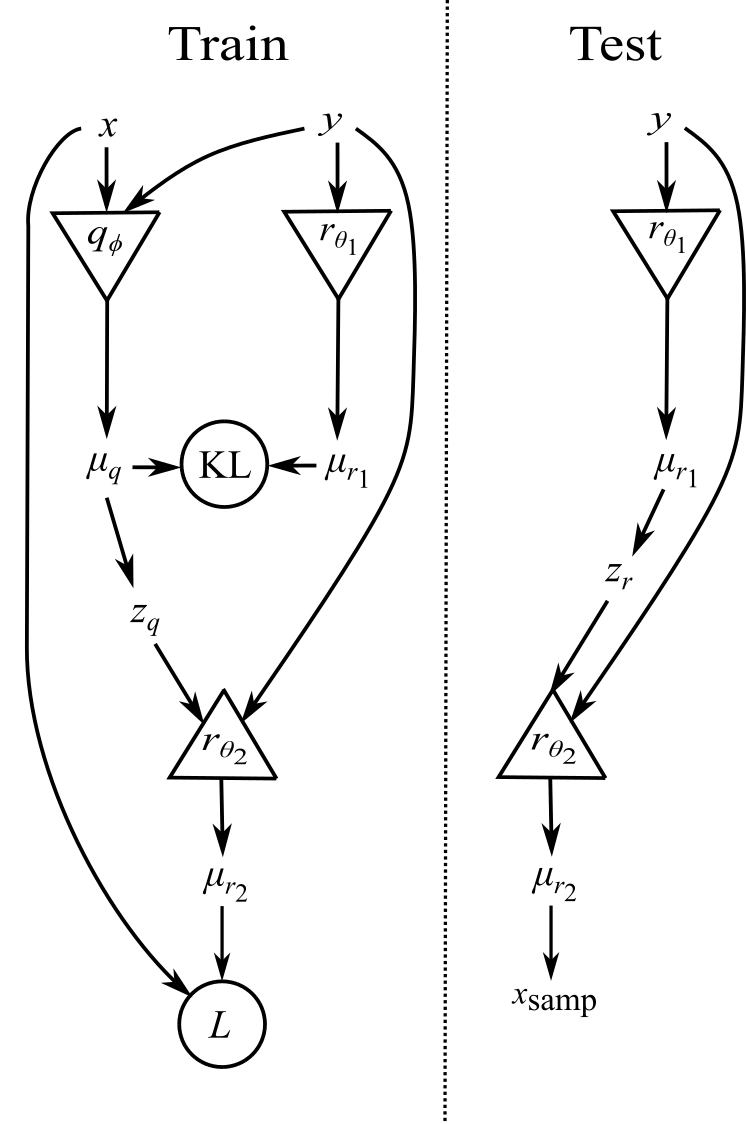
\includegraphics[width=0.95\columnwidth]{network_setup.png}
%    \caption{\label{fig:network_config} The configuration of the \ac{CVAE}
%neural network. During training (left-hand side), a training set of noisy
%\ac{GW} signals ($y$) and their corresponding true parameters ($x$) are given
%as input to encoder network $q_{\phi}$, while only $y$ is given to
%encoder network $r_{\theta_1}$. The \ac{KL}-divergence (Eq.~\ref{eq:kl})
%is computed between the encoder output latent space representations
%($\mu_q$ and $\mu_r$) forming one component of the total cost function. Samples
%($z_q$) from the $q_{\phi}$ latent space representation are generated and
%passed to the decoder network $r_{\theta_2}$ together with the original
%input data $y$. The output of the decoder ($\mu_x$) describes a distribution in
%the physical parameter space and the cost component $L$ is computed by
%evaluating that distribution at the location of the original input $x$.
%When performed in batches this scheme allows the computation of the total cost
%function Eq.~\ref{eq:cost3}. After having trained the network and
%therefore having minimised the cross-entropy $H$, we test (right-hand side)
%using only the $r_{\theta_1}$ encoder and the $r_{\theta_2}$
%decoder to produce samples ($x_{\text{samp}}$). These samples are drawn
%from the distribution $r_{\theta}(x|y)$ (Eq.~\ref{eq:latent_model})
%and accurately model the true posterior $p(x|y)$.}
%\end{figure}

%
% word count ~1500 - approx 9 words per line
%

%%%%%%%%%%%%%%%%%%%%%%%%%%%%%%%%%%%%%%%%%%%%%%%%%%%%%%%%%%%%%%%%%%%%%%
% RESULTS
%%%%%%%%%%%%%%%%%%%%%%%%%%%%%%%%%%%%%%%%%%%%%%%%%%%%%%%%%%%%%%%%%%%%%%
%
% results - here you would outline the process of comparison between the
% standard approach and the new one. Define training and test data and how Bilby
% is run on all test data for comparison. How do we then train our network. How
% do we then produce results on the test data. Here you refer to results plots
% but try to not make conclusion statements (just descriptive). Also include the
% speed analysis here.
%
%
% Intro to the results - what are we trying to do?
%

\section{Results}

We present results on $256$ multi-detector \ac{GW} test \ac{BBH}
waveforms in simulated advanced detector noise~\cite{aligo_noisecurves}
from the LIGO Hanford, Livingston and Virgo detectors. We compare between
variants of the existing Bayesian approaches and our \ac{CVAE} implementation
which we call \texttt{VItamin}. Posteriors produced by the \texttt{Bilby}
inference library~\cite{1811.02042} are used as a benchmark in order to assess
the efficiency and quality of our machine learning approach with the existing
methods for posterior sampling.

%
% describe the Bilby analysis 
%
For the benchmark analysis we assume that 9 parameters are
unknown\footnote{Our analysis omits the 6 additional parameters required to
model the spin of each \ac{BBH} component mass.}: the component masses
$m_1,m_2$, the luminosity distance $d_{\text{L}}$, the sky position
$\alpha,\delta$, the binary inclination $\Theta_{jn}$, the \ac{GW} polarisation
angle ${\psi}$, the time of coalescence $t_{0}$, and the phase at coalescence
$\phi_0$. For each parameter we use a uniform prior with the exception of
the declination and inclination parameters for which we use priors uniform in
$\cos\delta$ and $\sin\Theta_{jn}$ respectively. 
%The corresponding prior ranges
%are defined in Table~\ref{tab:prior_ranges} and result in an \ac{SNR}
%distribution that peaks at $\text{SNR}\approx 9$ and ranging between 0 and 75.
We use a sampling frequency of $256$~Hz, a time-series duration of 1 second, and
the waveform model used is \texttt{IMRPhenomPv2}~\cite{1809.10113} with a
minimum cutoff frequency of $20$Hz. For each input test waveform we run the
benchmark analysis using multiple sampling algorithms available within
\texttt{Bilby}. For each run and sampler we extract $\mathcal{O}(10^4)$
samples from the posterior on the 9 physical parameters.  

%
% the VItamin process
%
The \texttt{VItamin} training process uses as input $10^{7}$ whitened
waveforms corresponding to parameters drawn from the same priors as assumed for
the benchmark analysis. The waveforms are also of identical duration, sampling
frequency, and use the same waveform model as in the benchmark analysis.
The signals are whitened\footnote{The whitening is used primarily to
scale the input to a magnitude range more suitable to neural networks. The
\emph{true} \ac{PSD} does not have to be used for whitening, but training data
and test data must be contain signals that share the same \ac{PSD}.}
using the same advanced detector \acp{PSD}~\cite{aligo_noisecurves} as
assumed in the benchmark analysis. When each whitened waveform is placed
within a training batch it is given a unique detector Gaussian noise
realisation (after signal whitening this is simply zero mean, unit
variance Gaussian noise). The \texttt{VItamin} posterior results are produced by
passing each of our $256$ whitened noisy testing set of \ac{GW} waveforms
as input into the testing path of the pre-trained
\ac{CVAE}. For each input waveform we sample until we
have generated $10^4$ posterior samples on 7 physical parameters
$x=(m_1,m_2,d_{\text{L}},t_{0},\Theta_{jn},\alpha,\delta)$. We choose to
output a subset of the full 9-dimensional space to demonstrate that parameters
(such as $\phi_0$ and $\psi$ in this case) can (if desired) be
marginalised out within the \ac{CVAE} procedure itself, rather than after
training. 

%
% Corner plot results
%
\begin{figure*}
    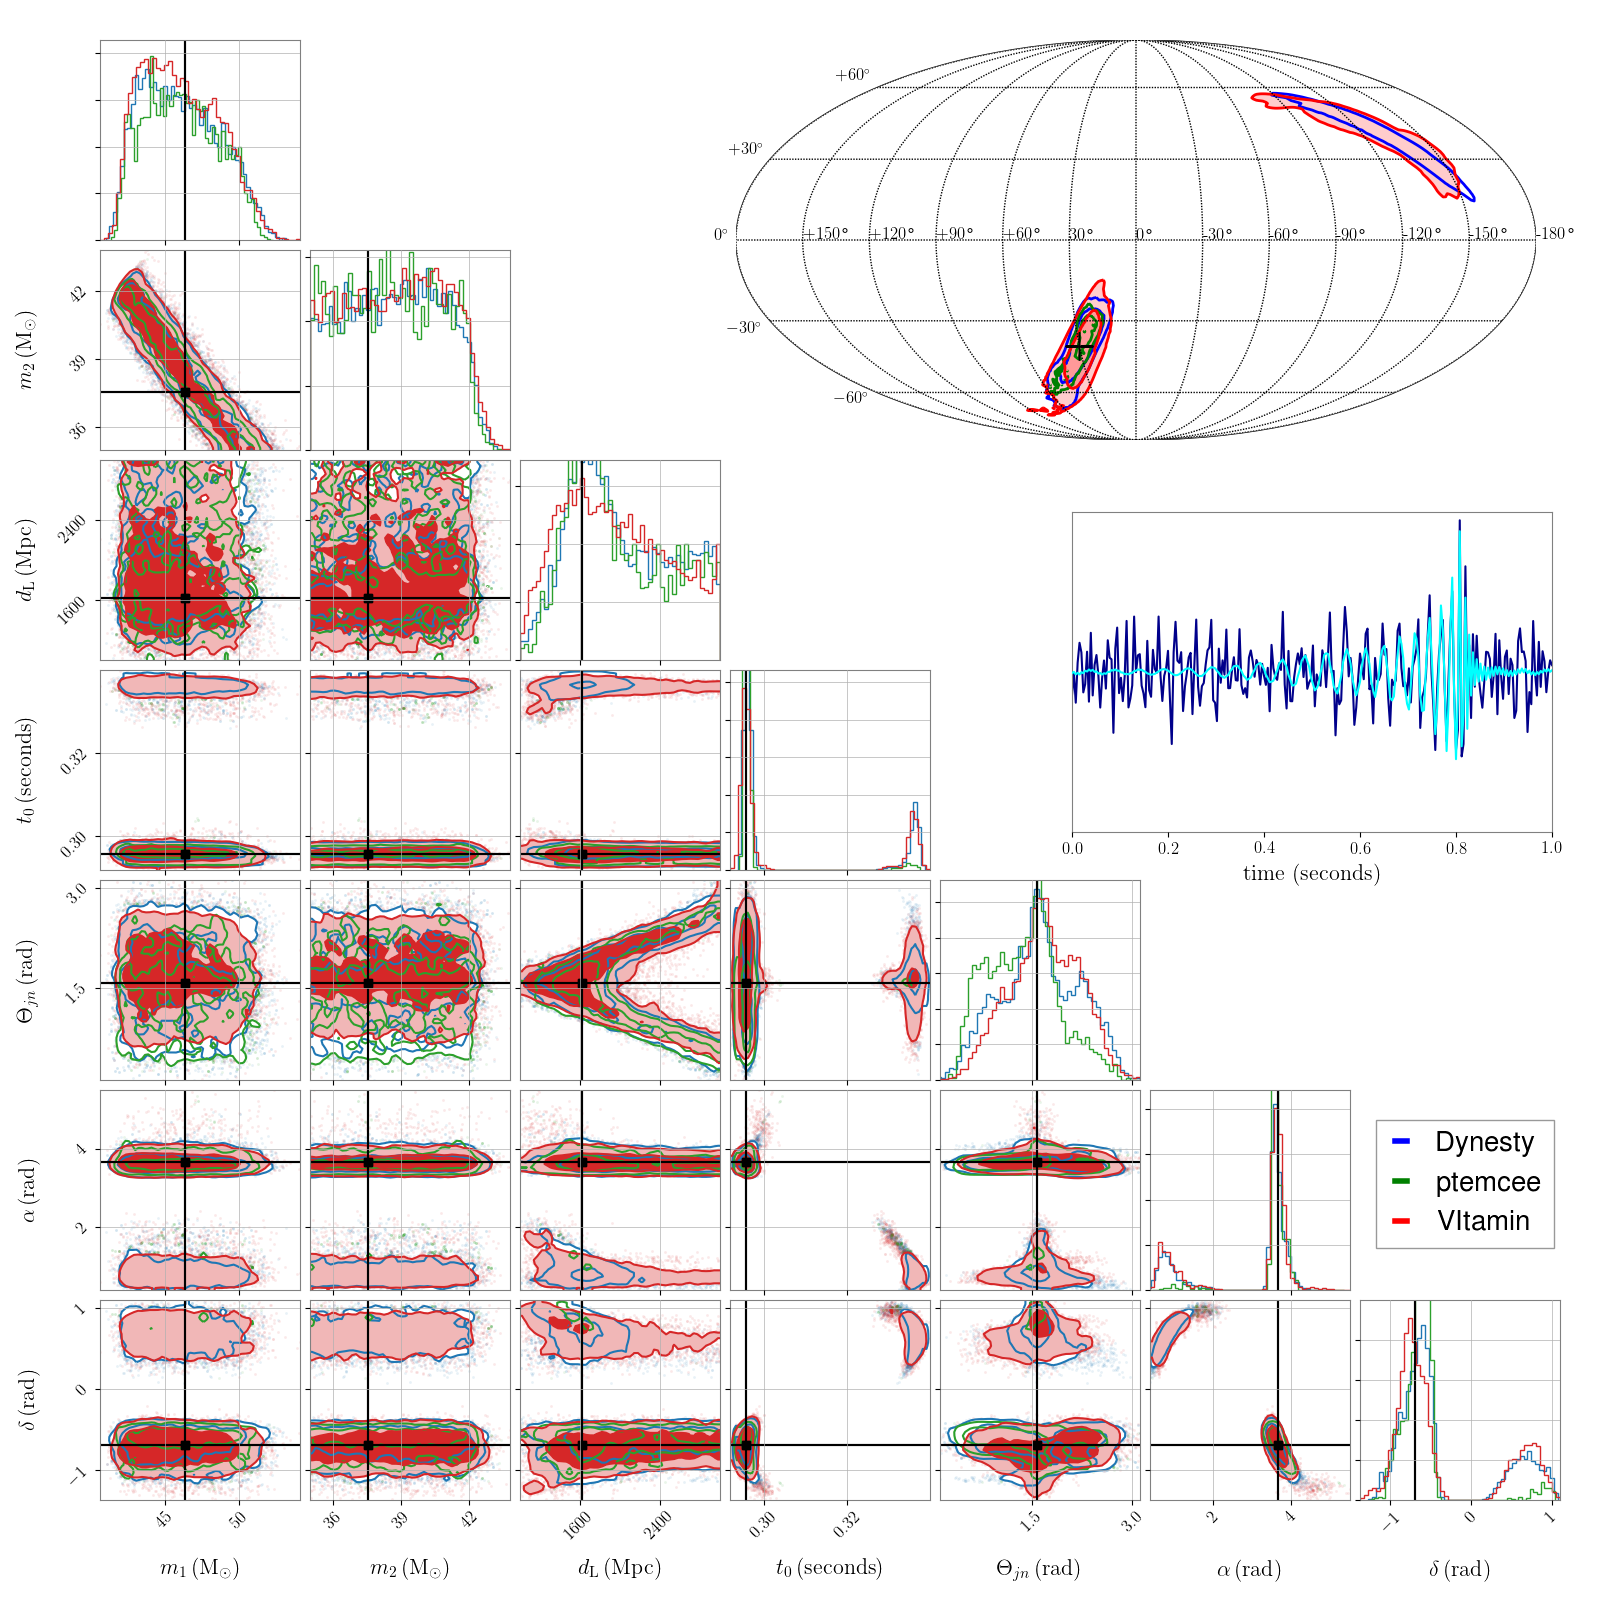
\includegraphics[width=\textwidth]{corner_testcase0.png}
    %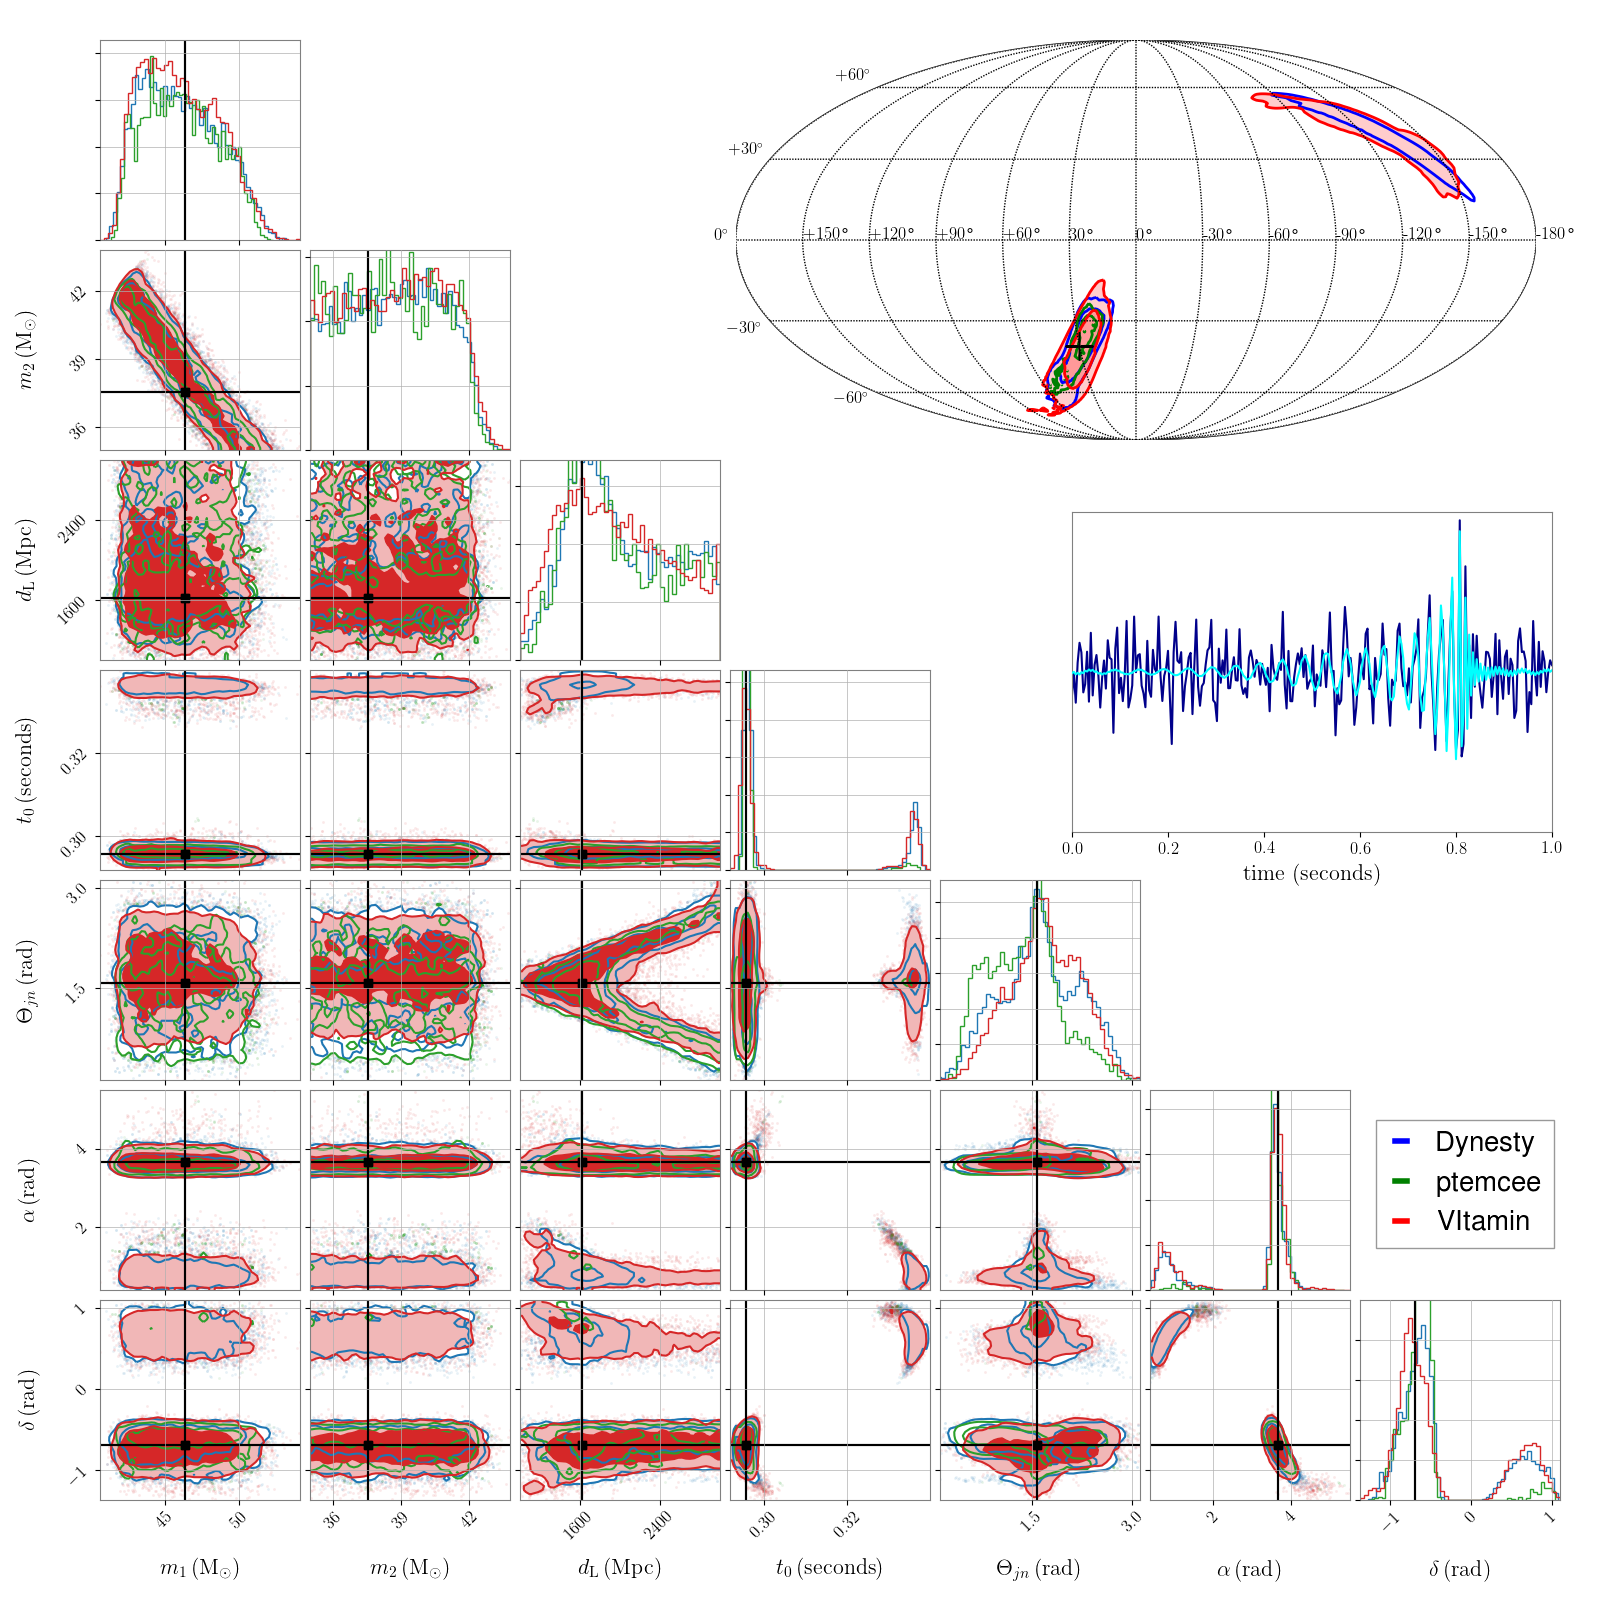
\includegraphics[scale=0.3]{corner_testcase0.png}
    \caption{\label{fig:corner_plot} Corner plot showing one and two-dimensional
marginalised posterior distributions on the \ac{GW} parameters for one
example test dataset. Filled red contours represent the
two-dimensional joint posteriors obtained from \texttt{VItamin} and
solid blue and green contours are the corresponding posteriors
output from our benchmark analyses (using the \texttt{Dynesty} and \texttt{ptemcee}
samplers within \texttt{Bilby}). In each case, the contour boundaries enclose
$68,90$ and $95\%$ probability. One dimensional histograms of the posterior
distribution for each parameter from both methods are plotted along the
diagonal. Black vertical and horizontal lines denote the true parameter
values of the simulated signal. At the top of the figure we include a Mollweide
projection of the sky location posteriors from all three analyses. All results
presented in this letter correspond to a three-detector configuration but for
clarity we only plot the H1 whitened noisy time-series $y$ and the noise-free
whitened signal (in blue and cyan respectively) to the right of the figure. The
test signal was simulated with an optimal multi-detector signal-to-noise ratio of
17.2.} 
\end{figure*}

%
% discuss the corner plot results
%
We can immediately illustrate the accuracy of our machine learning predictions
by directly plotting 2 and one-dimensional marginalised posteriors generated
using the output samples from our \texttt{VItamin} and \texttt{Bilby}
approaches superimposed on each other. We show this for one example test
dataset in Fig.~\ref{fig:corner_plot} where strong agreement between 2
\texttt{Bilby} samplers (\texttt{Dynesty} in blue, and \texttt{ptemcee} in green) and the
\ac{CVAE} (red) is clear. It is also evident that whilst we refer to the
\texttt{Bilby} sampler results as benchmark cases, different existing samplers
do not perfectly agree with each other. For each of our 256 test cases we see
equivalent levels of disparity between pairs of benchmark samplers \emph{and}
between any benchmark sampler and our \ac{CVAE} results.  In \cite{1909.06296} we also 
show the results of 2 statistical tests (the \ac{PP} plot test and
\ac{KL}-divergence tests) performed on the entire test dataset and between all
samplers (\texttt{Dynesty}, \texttt{ptemcee}, \texttt{CPNest}, \texttt{emcee}, and \texttt{VItamin}).

%
% mention the p-p plot and KL distribution results
%
%In
%both tests the quality of the \texttt{VItamin} results are indistinguishable from the
%benchmark samplers. The \ac{PP} plot results specifically indicate that the
%Bayesian one-dimensional marginalised posteriors from each approach are
%self-consistent from a frequentist perspective (e.g., the true values lie
%within the $X\%$ confidence interval for $X\%$ of the test cases). The second
%test computes the distribution of \ac{KL}-divergences between posteriors
%conditioned on the same test data $y$ from pairs of samplers. In all cases this
%measure of ``distribution similarity'' between \texttt{VItamin} and any particular
%benchmark sampler is entirely consistent with the distribution between that
%benchmark sampler and any other.   

%
% discuss the speed of the analysis
%
The dominating computational cost of running \texttt{VItamin} lies in the
training time, which takes $\mathcal{O}(1)$ day to complete. We
stress that once trained, there is no need to retrain the network unless the
user wishes to use different priors $p(x)$ or assume different noise
characteristics. Run-time for the benchmark samplers is defined as the time to complete their
analyses when configured using the parameter choices. For \texttt{VItamin}, this time is defined as
the total time to produce $10^4$ samples. For our test case of \ac{BBH} signals
\texttt{VItamin} produces samples from the posterior at a rate which is $\sim
6$ orders of magnitude faster than our benchmark analyses using current
inference techniques. 

%\chris{One more thing to add, especially if the other KL, AD, and PP plots
%aren't convincing, is a plot displaying 1D confidence bounds compared between
%bilby and VItamin. Imagine a plot with the x-axis as distance and the y-axis
%steps through test data with increasing true distance. for each test data you
%plot 2 error bars horizontally (one for bilby and one for VItamin) spanning the
%range of 90\% confidence. You would hopefully get nearly identical pairs of
%errorbars stacked vertically. Technically you could do this for all parameters
%(and you should) but we might only put one of the plots in the paper (if at
%all).}

%
% I feel the need, the need for speed, table
% 
%\begin{table}
%\centering
%\caption{Durations required to produce samples from each of
%the different posterior sampling approaches.}
%\begin{tabular}[t]{lcccc} 
%\toprule
%\multirow{2}{*}{sampler} & \multicolumn{3}{c}{run time (seconds)} & \multirow{2}{*}{ratio
%$\displaystyle\frac{\tau_{\text{VItamin}}}{\tau_{X}}$} \\
%& min & max & median & \\
%\hline
%\texttt{Dynesty}\footnote{The benchmark samplers all produced
%$\mathcal{O}(10000)$ samples dependent on the default sampling parameters
%used.}~\cite{dynesty} & 11795 & 29838 & 19400
%\footnote{We note that there are a growing number of specialised
%techniques~\cite{2016PhRvD..94d4031S,2019PhRvD..99h4026W,2019PhRvD.100d3030T}
%designed to speed up traditional sampling algorithms that could be used to
%reduce the runtimes quoted here by $\mathcal{O}(1-2)$ orders of magnitude.}
%\footnote{The reader may note that benchmark sampler run times are a few orders
%of magnitude lower than what is typical of a complete \ac{BBH} analysis
%($\mathcal{O}(10^{4} -10^{5})$ seconds). This is primarily due our use of a
%reduced parameter space, low sampling rate and choice of sampler
%hyperparameters.} 
%& $5.2\times 10^{-6}$ \\
%\texttt{emcee}~\cite{emcee} & 18838 & 69272 & 32070 & $3.1\times 10^{-6}$ \\
%\texttt{ptemcee}~\cite{ptemcee} & 17124 & 37446 & 24372 & $4.1\times 10^{-6}$ \\
%\texttt{CPNest}~\cite{cpnest} & 9943 & 53315 & 26202 & $3.8\times 10^{-6}$ \\
%\texttt{VItamin}\footnote{For the \texttt{VItamin} sampler $10000$ samples are
%produced as representative of a typical posterior. The run time is independent
%of the signal content in the data and is therefore constant for all test cases.} & \multicolumn{3}{c}{\bm{$1\times 10^{-1}$}} & 1 \\
%\botrule
%\end{tabular}
%\label{Tab:speed}
%\end{table}

%
% word count ~960 - approx 9.6 words per line
%

%%%%%%%%%%%%%%%%%%%%%%%%%%%%%%%%%%%%%%%%%%%%%%%%%%%%%%%%%%%%%%%%%%%%%%
% CONCLUSIONS
%%%%%%%%%%%%%%%%%%%%%%%%%%%%%%%%%%%%%%%%%%%%%%%%%%%%%%%%%%%%%%%%%%%%%%
%
% conclusions - now draw conclusions about the quality of the comparison
% results. Highlight the current limitations but also highlight the importance of
% this for the GW field (multi-detector is easy, additional parameters are easy,
% longer datasets may be a challenge regarding GPU memory?, we don't have to
% assume a noise model if we inject training data into real noise, we do rely on
% well defined signal models, EM-follow up in very low latency, can we use
% transfer learning if we want to retrain, ...) End with broader statements about
% inference in other fields and how this is applicable across the sciences.
%
% recap and main result
%
\section{Conclusions}

%In this paper we have demonstrated that we are able to reproduce, to a high
%degree of accuracy, Bayesian posterior probability distributions generated
%through machine learning. This is accomplished using a \ac{CVAE} trained on
%simulated \ac{GW} signals and does not require the input of precomputed
%posterior estimates. We have demonstrated that our neural network model, which
%when trained, can reproduce complete and accurate posterior estimates in
%a fraction of a second, achieves the same quality of results as the
%trusted benchmark analyses used within the LIGO-Virgo Collaboration.

%
% CBC implications and why this is a game-changer - speed for EM followup
%
The significance of our results is most evident in the orders of magnitude
increase in speed over existing algorithms. We have demonstrated the approach
using \ac{BBH} signals but with additional work to increase sample rate
and signal duration, the method can also be extended for application to
signals from \ac{BNS} mergers (e.g., GW170817~\cite{PhysRevLett.119.161101},
and GW190425~\cite{2020ApJ...892L...3A}) and \ac{NSBH} systems where
improved low-latency alerts will be especially pertinent. By using our
approach, parameter estimation speed will no longer be limiting
factor\footnote{A complete low-latency pipeline includes a number of
steps. The process of \ac{GW} data acquisition is followed by the transfer of
data. There is then the corresponding candidate event identification,
parameter estimation analysis, and the subsequent communication of results to
the \ac{EM} astronomy community after which there are physical aspects such as
slewing observing instruments to the correct pointing.} in observing the prompt
\ac{EM} emission expected on shorter time scales than is achievable with
existing \ac{LVC} analysis tools such as Bayestar~\cite{2016PhRvD..93b4013S}.

%
% CBC implications and why this is a game-changer - faster, modular
%
The predicted number of future detections of \ac{BNS} mergers ($\sim
180$~\cite{2018LRR....21....3A}) will severely strain the \ac{GW} community's
current computational resources using existing Bayesian methods. We anticipate
that future iterations of our approach will provide full-parameter estimation
on all classes of \ac{CBC} signals in $\mathcal{O}(1)$ second on single
\acp{GPU}. Our trained network is also modular, and can be shared and used
easily by any user to produce results. The specific analysis described in this
paper assumes a uniform prior on the signal parameters. However, this is a
choice and the network can be trained with any prior the user demands, or users
can cheaply resample accordingly from the output of the network trained on the
uniform prior. We also note that our method will be invaluable for population
studies since populations may now be generated and analysed in a fully-Bayesian
manner on a vastly reduced time scale. Our work can naturally be extended to include the full range of \ac{CBC} signal types but also to any and all other parameterised \ac{GW}
signals and to analyses of \ac{GW} data beyond that of ground based
experiments. Given the abundant benefits of this method, we hope that a variant
of this of approach will form the basis for future \ac{GW} parameter
estimation.
 

%
% Non Gaussian noise and the final statement
%
%In reality, \ac{GW} detectors are affected by non-Gaussian noise artefacts and
%time-dependent variation in the detector noise \ac{PSD}. Existing methods
%incorporate a parameterised \ac{PSD} estimation into their
%inference~\cite{2015PhRvD..91h4034L}. To account for these and to exploit the
%``likelihood-free'' nature of the \ac{CVAE} approach, we could re-train our
%network at regular intervals using samples of real detector noise (preferably
%recent examples to best reflect the state of the detectors). In this case
%we could also apply transfer learning to speed up each training instance based
%on the previously trained network state.  Alternatively, since the \ac{PSD} is
%an estimated quantity, we could marginalise over its uncertainty by providing
%training data whitened by samples drawn from a distribution of possible
%\acp{PSD}. Our work can naturally be extended to include the full range of
%\ac{CBC} signal types but also to any and all other parameterised \ac{GW}
%signals and to analyses of \ac{GW} data beyond that of ground based
%experiments. Given the abundant benefits of this method, we hope that a variant
%of this of approach will form the basis for future \ac{GW} parameter
%estimation.

%
% word count ~620
%

\section*{Broader Impact}



%
% future work, current limitations and prospects
%
Our work may be applied to a wide range of applications within the 
\ac{GW} community (population studies, rapid \ac{EM} partner 
astronomer \ac{GW} signal sky localisation alerts, etc.). In terms of  
reliability, our \ac{CVAE} approach is currently just as 
reliant on accurate noise and signal models as existing techniques. 
However, there is the potential to step away from this reliance in the 
future and to make our results more robust against these important 
effects than is possible with existing techniques.

In reality, \ac{GW} detectors are affected by non-Gaussian noise artefacts and
time-dependent variation in the detector noise \ac{PSD}. Existing methods
incorporate a parameterised \ac{PSD} estimation into their
inference~\cite{2015PhRvD..91h4034L}. To account for these and to exploit the
``likelihood-free'' nature of the \ac{CVAE} approach, we could re-train our
network at regular intervals using samples of real detector noise (preferably
recent examples to best reflect the state of the detectors). In this case
we could also apply transfer learning to speed up each training instance based
on the previously trained network state.  Alternatively, since the \ac{PSD} is
an estimated quantity, we could marginalise over its uncertainty by providing
training data whitened by samples drawn from a distribution of possible
\acp{PSD}.

\begin{ack}
%
% acknowledge people and funding agencies
%
%\section{Acknowledgements.}
%
We would like to acknowledge valuable input from the LIGO-Virgo Collaboration,
specifically from Will Farr, Tom Dent, Jonah Kanner, Alex Nitz, Colin Capano 
and the parameter estimation 
and machine-learning working groups. We would additionally like to thank Szabi 
Marka for posing this challenge to us and the journal referees for their 
helpful and constructive comments. We thank Nvidia for the generous donation 
of a Tesla V-100 GPU used in addition to \ac{LVC} computational resources. 
The authors also gratefully acknowledge the Science and Technology Facilities 
Council of the United Kingdom. CM and SH are supported by the Science and 
Technology Research Council (grant No.~ST/~L000946/1) and the European 
Cooperation in Science and Technology (COST) action CA17137. FT acknowledges 
support from Amazon Research and  EPSRC grant EP/M01326X/1, and RM-S EPSRC 
grants EP/M01326X/1, EP/T00097X/1 and EP/R018634/1. 
\end{ack}

%\bibliographystyle{apsrev4-1}
\bibliographystyle{abbrv}
\bibliography{references}% Produces the bibliography via BibTeX.


\end{document}
